% \documentclass[12pt, twoside]{article}
\usepackage[letterpaper, margin=1in, headsep=0.2in]{geometry}
\setlength{\headheight}{0.6in}
%\usepackage[english]{babel}
\usepackage[utf8]{inputenc}
\usepackage{microtype}
\usepackage{amsmath}
\usepackage{amssymb}
%\usepackage{amsfonts}
\usepackage[nomessages]{fp} %\FPeval{\var-name}{2*sin(pi/6)}
\usepackage{siunitx} %units in math. eg 20\milli\meter
\usepackage{yhmath} % for arcs, overparenth command
\usepackage{tikz} %graphics
\usetikzlibrary{quotes, angles, arrows, arrows.meta}
\usepackage{graphicx} %consider setting \graphicspath{{images/}}
\usepackage{parskip} %no paragraph indent
\usepackage{enumitem}
\usepackage{multicol}
\usepackage{venndiagram}

\usepackage{fancyhdr}
\pagestyle{fancy}
\fancyhf{}
\renewcommand{\headrulewidth}{0pt} % disable the underline of the header
\raggedbottom
\hfuzz=2mm %suppresses overfull box warnings

\usepackage{hyperref}

\fancyhead[LE]{\thepage}
\fancyhead[RO]{\thepage \\ Name: \hspace{4cm} \,\\}
\fancyhead[LO]{BECA / Dr. Huson / Geometry\\*  Unit 4: Volume and polyhedra \\* 20 October 2022}

\begin{document}

\subsubsection*{4.8 Homework: Density of 3-dimensional objects, weight and cost}
\begin{enumerate}
\item Do Now: Complete the four problems in the Graspable Math activity linked above. Paste a cropped screenshot of the fourth problem here. It should look like the modelled solution below.

\item \emph{Density} is a ratio that maps proportional variables having different units. For example, weight per volume or population per area. \\[0.5cm]
Find the weight of a volume of water of 100 cubic feet if the density of water is 62.4 pounds per cubic feet.  \\[0.5cm]
$W=V \times D$\\
$W=100 \times 62.4$\\
$W=6,240$ pounds \\[0.5cm]
Find the weight of 125 cubic feet of water.

\item Find the volume of a rectangular prism volume of water. Its length is $l=20$ feet, its height $h=12$ feet, and depth is $w=10$ feet. Start with the equation \\[0.5cm]
$V = l \times w \times h$
  \begin{flushright}
    \begin{tikzpicture}[scale=1.25]
      \draw [-, thick] (0,0)--(4,0)--(4,2)--(0,2)--cycle;
      \draw [-, thick] (0,2)--(0.5,2.75)--(4.5,2.75)--(4,2);
      \draw [-, thick] (4,0)--(4.5,0.75)--(4.5,2.75);
      \node at (4.75, 1.75){$12$};
      \node at (2, -0.25){$20$};
      \node at (4.5, 0.25){$10$};
    \end{tikzpicture}
  \end{flushright}

\item A parallelogram is shown on the $x$-$y$ plane having a base $b=4.25$ and height $h=7.0$. 
  \begin{multicols}{2}
    Find its area, showing the calculation.
      \begin{flushright}
      \begin{tikzpicture}[scale=.635]
        %\draw [help lines] (-1,-1) grid (9,6);
        \draw [thick, ->] (-1.2,0) -- (7.4,0) node [below right] {$x$};
        \draw [thick, ->] (0,-1.2)--(0,6.4) node [left] {$y$};
        \draw [<->, thick] (1.5,1)--(1.5,5);
        \draw [-, thick] (2,1)--(4.75,1)--(5.75,5)--(3,5)--cycle;
        \node at (3.5,1)[below]{$4.25$};
        \node at (1.5,3)[left]{$7.0$};
      \end{tikzpicture}
      \end{flushright}
  \end{multicols} 

\item The $\triangle ABC$ is shown below with $A(3,1)$, $B(7,1)$, and $C(2,6)$. The length of the base of the triangle is $AB=4$.
  \begin{multicols}{2}
    \begin{enumerate}
      \item Find the height $h$.
      \item Find the triangle's area, showing the calculation. \vspace{2cm}
      \end{enumerate}
      \begin{flushright}
      \begin{tikzpicture}[scale=.635]
        \draw [help lines] (-1,-1) grid (9,7);
        \draw [thick, ->] (-1.2,0) -- (9.4,0) node [below right] {$x$};
        \draw [thick, ->] (0,-1.2)--(0,7.4) node [left] {$y$};
        \draw [<->, thick] (1.5,1)--(1.5,6);
        \draw [-, thick] (3,1)--(7,1)--(2,6)--cycle;
        \draw [-, dashed] (7,1)--(6,6)--(2,6);
        \draw [fill] (3,1) circle [radius=0.05] node[below] {$A$};
        \draw [fill] (7,1) circle [radius=0.05] node[below] {$B$};
        \draw [fill] (2,6) circle [radius=0.05] node[above right] {$C$};
        \node at (5,1)[below]{$4$};
        \node at (0.5,3)[right]{$h$};
      \end{tikzpicture}
      \end{flushright}
  \end{multicols} 

\item Find the width of the base of a rectangle with area $A=75$ and height $h=15$. Start with the form (use $b$ or $x$): \\[0.5cm]
$A = b \times h = 75$
  \begin{flushright}
  \begin{tikzpicture}[scale=1.25]
    \draw [-, thick] (0,0)--(2,0)--(2,6)--(0,6)--cycle;
    \node at (2.5, 3){$15$};
    \node at (1, -0.5){$?$};
    \node at (1, 3){$75$};
  \end{tikzpicture}
  \end{flushright}

\item Find the height of the $\triangle BLM$, having an area of $A=42$ and base $BL=7$.
  \begin{multicols}{2}
    Start by substituting values in the area formula: \\[0.5cm]
    $\displaystyle A = \frac{1}{2} bh = 42$ \vspace{2cm}
      \begin{flushright}
      \begin{tikzpicture}[scale=.635]
        %\draw [help lines] (-1,-1) grid (9,6);
        \draw [thick, ->] (-1.2,0) -- (9.4,0) node [below right] {$x$};
        \draw [thick, ->] (0,-1.2)--(0,8.4) node [left] {$y$};
        \draw [<->, thick] (1.5,1)--(1.5,7);
        \draw [-, thick] (2,1)--(6,1)--(5,7)--cycle;
        \draw [-, dashed] (6,1)--(9,7)--(5,7);
        \draw [fill] (2,1) circle [radius=0.05] node[below] {$B$};
        \draw [fill] (6,1) circle [radius=0.05] node[below] {$L$};
        \draw [fill] (5,7) circle [radius=0.05] node[above left] {$M$};
        \node at (4,1)[below]{$7$};
        \node at (1.5,4)[left]{$h$};
      \end{tikzpicture}
      \end{flushright}
  \end{multicols}

\item The rectangular prism shown has a volume of $V=1815$ cubic centimeters. Its base measures $l=12.5$ cm by $w=8.8$ cm. \\[0.5cm]
Find its height in centimeters. Begin by writing the following formula with values substituted: \\[0.5cm]
$V = l \times w \times h = 1815$
\begin{flushright}
  \begin{tikzpicture}[scale=1]
    \draw [-, thick] (0,0)--(3,0)--(3,4)--(0,4)--cycle;
    \draw [-, thick] (0,4)--(0.5,4.75)--(3.5,4.75)--(3,4);
    \draw [-, thick] (3,0)--(3.5,0.75)--(3.5,4.75);
    \node at (3.75, 2.75){$h$};
    \node at (1.5, -0.25){$12.5$};
    \node at (4, 0.25){$8.8$};
  \end{tikzpicture}
\end{flushright}

\item Find the length of the base of a triangle with area $A=30$ and height $h=6 \frac{2}{3}$. Start with the form (use $b$ or $x$): \\[0.5cm]
$A = \frac{1}{2} \times b \times h = 30$
  \begin{flushright}
  \begin{tikzpicture}[scale=1.25]
    \draw [-, thick] (-1,0)--(3,0)--(2.5,3.5)--cycle;
    \node at (3.3, 1.5){$\displaystyle 6 \frac{2}{3}$};
    \node at (1, -0.5){$?$};
    \node at (1.5, 1){$A = 30$};
  \end{tikzpicture}
  \end{flushright}

\item Find the area of the $\triangle ABC$, shown below, with $A(1,2)$, $B(7,4)$, and $C(4,8)$. 
  \begin{multicols}{2}
    Hint: Subtract the areas of the three right triangles from the area of the red square.
      \begin{flushright}
      \begin{tikzpicture}[scale=.635]
        \draw [help lines] (-1,-1) grid (9,9);
        \draw [thick, ->] (-1.2,0) -- (9.4,0) node [below right] {$x$};
        \draw [thick, ->] (0,-1.2)--(0,9.4) node [left] {$y$};
        %\draw [<->, thick] (0.5,1)--(0.5,5);
        \draw [-, thick] (1,2)--(7,4)--(4,8)--cycle;
        \draw [-, thick, red] (1,2)--(7,2)--(7,8)--(1,8)--cycle;
        \draw [fill] (1,2) circle [radius=0.05] node[below left] {$A$};
        \draw [fill] (7,4) circle [radius=0.05] node[right] {$B$};
        \draw [fill] (4,8) circle [radius=0.05] node[above right] {$C$};
        \node at (4,2)[below]{$6$};
        \node at (0.2,5)[right]{$6$};
      \end{tikzpicture}
      \end{flushright}
  \end{multicols} 

\item A rectangular prism has a square base. Its volume is $V=162$ cubic centimeters and its height is $h=8$ cm.
  \begin{multicols}{2}
    Calculate the dimensions of its base.
    \begin{flushright}
      \begin{tikzpicture}[scale=1]
        \draw [-, thick] (0,0)--(3,0)--(3,4)--(0,4)--cycle;
        \draw [-, thick] (0,4)--(0.5,4.75)--(3.5,4.75)--(3,4);
        \draw [-, thick] (3,0)--(3.5,0.75)--(3.5,4.75);
        \node at (3.75, 2.75){$8$};
        \node at (1.5, -0.25){$x$};
        \node at (3.5, 0.25){$x$};
      \end{tikzpicture}
    \end{flushright}
  \end{multicols}

\item Do Now: Find the area of a triangle with base $b=12.5$ and height $h=8.4$. Use the Graspable Math activity linked above. Paste a cropped screenshot of the first problem here. It should look like the modelled solution below.
\begin{itemize}[label=$\square$]
  \item Copy expressions (drag the handle on the left of the formula)
  \item Substitute values (drag the variable onto the formula)
  \item Show/hide steps (show the substitution, final line, and key steps)
  \item Copy/paste screenshot: command-control-shift-4 (Mac)
\end{itemize}
\begin{flushright}
  \includegraphics[width=8cm]{../graphics/04model-solution.png}
\end{flushright}

\item Find the area of a semi-circle with radius $r=7.5$. Paste a cropped screenshot of the Graspable Math. Compare your format to the model solution.
\item \vspace{4cm}
\begin{flushright}
  \includegraphics[width=10cm]{../graphics/04asolution.png}
\end{flushright}

\item Find the population density of Queens, New York. Paste a cropped screenshot of the Graspable Math. Make a copy of the formula and show the substitution step.
\vspace{4cm}
\begin{flushright}
  \includegraphics[width=9cm]{../graphics/04solution.png}
\end{flushright}

\item Find the area of rectangle $ABCD$ having length $l=11$ and width $w=3 \frac{3}{5}$. Start with a formula of this form, substituting the given values: \\[0.5cm]
$A = l \times w$
  \begin{flushright}
  \begin{tikzpicture}[scale=1.25]
    \draw [-, thick] (0,0)--(4.5,0)--(4.5,2)--(0,2)--cycle;
    \draw [fill] (0,0) circle [radius=0.05] node[left]{$A$};
    \draw [fill] (4.5,0) circle [radius=0.05] node[right]{$B$};
    \draw [fill] (4.5,2) circle [radius=0.05] node[right]{$C$};
    \draw [fill] (0,2) circle [radius=0.05] node[left]{$D$};
    \node at (5, 1){$3 \frac{3}{5}$};
    \node at (2.25, -0.5){$11$};
    %\node at (2.25, 1){$A = 15$};
  \end{tikzpicture}
  %https://graspablemath.com/canvas?load=_fa182d9d9d78d850
  \end{flushright}

\item Find the weight of a volume of water of 18 cubic feet given that the density of water is 62.4 pounds per cubic foot.  \\[0.5cm]
$W=V \times D$
%https://graspablemath.com/canvas?load=_4fe25c69e45fccbd

\item The $\triangle ABC$ is shown below with $A(4,1)$, $B(7,1)$, and $C(2,6)$. The length of the base of the triangle is $AB=3$.
  \begin{multicols}{2}
    \begin{enumerate}
      \item Write down the height $h$.
      \item Find the triangle's area, showing the substitution into the area formula.\\[0.25cm]
      $A=\frac{1}{2}bh$ \vspace{2cm}
      \end{enumerate}
      \begin{flushright}
      \begin{tikzpicture}[scale=.635]
        \draw [help lines] (-1,-1) grid (9,7);
        \draw [thick, ->] (-1.2,0) -- (9.4,0) node [below right] {$x$};
        \draw [thick, ->] (0,-1.2)--(0,7.4) node [left] {$y$};
        \draw [<->, thick] (1.5,1)--(1.5,6);
        \draw [-, thick] (4,1)--(7,1)--(2,6)--cycle;
        \draw [-, dashed] (7,1)--(5,6)--(2,6);
        \draw [fill] (4,1) circle [radius=0.05] node[below] {$A$};
        \draw [fill] (7,1) circle [radius=0.05] node[below] {$B$};
        \draw [fill] (2,6) circle [radius=0.05] node[above right] {$C$};
        \node at (5.5,1)[below]{$3$};
        \node at (0.5,3)[right]{$h$};
      \end{tikzpicture}
      \end{flushright}
      %https://graspablemath.com/canvas?load=_7190d54aa454877d
  \end{multicols}

\item Find the volume of a pyramid having a square base 3 units on each side, $s=3$, and a height of $h=4$. Show the substitution in the volume formula for full credit. \\[0.5cm]
$\displaystyle V = \frac{1}{3} s^2 h$
  \begin{flushright}
    \includegraphics[width=9cm]{../graphics/04pyramid.png}
    %https://graspablemath.com/canvas?load=_84b1e82deef48a75
  \end{flushright}

\item The American Eagle gold coin is minted by the US Treasury. The one ounce coin has a radius of about $r=16$ millimeters and thickness $h=3$ mm. Given a density of $D = 0.014$ grams per cubic millimeter, find the coin's volume and weight. \\[0.25cm]
Show the substitution into both formulas for full credit.\\[0.5cm]
$\displaystyle V = \pi r^2 h$ and $W=VD$
  \begin{flushright}
    \includegraphics[width=7cm]{../graphics/04bcoin.png}
    %https://graspablemath.com/canvas?load=_845e39ea582acd9e
  \end{flushright}
  
\item A parallelogram is shown on the $x$-$y$ plane having a base $b=14.5$, unknown height $h$, and area $A=348$. Find the height. 
  \begin{multicols}{2}
    Show the area formula with substituted values for full credit.
      \begin{flushright}
      \begin{tikzpicture}[scale=.8]
        %\draw [help lines] (-1,-1) grid (9,6);
        \draw [thick, ->] (-1.2,0) -- (7.4,0) node [below right] {$x$};
        \draw [thick, ->] (0,-1.2)--(0,6.4) node [left] {$y$};
        \draw [<->, thick] (1.5,1)--(1.5,5);
        \draw [-, thick] (2,1)--(4.75,1)--(5.75,5)--(3,5)--cycle;
        \node at (3.5,1)[below]{$14.5$};
        \node at (1.5,3)[left]{$h$};
        \node at (3.7,3)[]{$A=348$};
      \end{tikzpicture}
      \end{flushright}
  \end{multicols} 

\item Find the population density of Brooklyn, New York (Kings County) in people per square mile.\\[0.5cm]
Population estimate July 1, 2019: 2,559,903\\[0.25cm]
Land area in square miles: 69.4
\begin{flushright}
  \includegraphics[width=8cm]{../graphics/04Brooklyn.png}\\
  Source: US Census (census.gov)
  %https://graspablemath.com/canvas?load=_0b517bab59c981c7
\end{flushright}

\item The rectangular prism shown has a volume of $V=9911$ cubic centimeters. Its base measures $l=22$ centimeters by $w=13.25$ cm. \\[0.5cm]
Find its height in centimeters. For credit, begin by writing the volume formula with values substituted.
\begin{flushright}
  \begin{tikzpicture}[scale=1]
    \draw [-, thick] (0,0)--(3,0)--(3,4)--(0,4)--cycle;
    \draw [-, thick] (0,4)--(0.5,4.75)--(3.5,4.75)--(3,4);
    \draw [-, thick] (3,0)--(3.5,0.75)--(3.5,4.75);
    \node at (3.75, 2.75){$h$};
    \node at (1.5, -0.25){$22$};
    \node at (4, 0.25){$13.25$};
  \end{tikzpicture}
  %https://graspablemath.com/canvas?load=_21d5199065c209a4
\end{flushright}

\item Find the radius of a sphere having a volume of 6367.4 cubic inches. Round to \emph{the nearest tenth of an inch}. Show the substitution in the volume formula for full credit. \\[0.5cm]
$\displaystyle V = \frac{4}{3} \pi r^3$
  \begin{flushright}
    \includegraphics[width=8cm]{../graphics/04sphere.png}
    %https://graspablemath.com/canvas?load=_7f185d285c634826
  \end{flushright}

\item Find the area of rectangle $ABCD$ having length $l=18$ and width $w=6 \frac{1}{4}$. Start with a formula of this form, substituting the given values: \\[0.5cm]
$A = l \times w$
  \begin{flushright}
  \begin{tikzpicture}[scale=1.25]
    \draw [-, thick] (0,0)--(4.5,0)--(4.5,2)--(0,2)--cycle;
    \draw [fill] (0,0) circle [radius=0.05] node[left]{$A$};
    \draw [fill] (4.5,0) circle [radius=0.05] node[right]{$B$};
    \draw [fill] (4.5,2) circle [radius=0.05] node[right]{$C$};
    \draw [fill] (0,2) circle [radius=0.05] node[left]{$D$};
    \node at (5, 1){$6 \frac{1}{4}$};
    \node at (2.25, -0.5){$18$};
    %\node at (2.25, 1){$A = 15$};
  \end{tikzpicture}
  %https://graspablemath.com/canvas?load=_fa182d9d9d78d850
  \end{flushright}

\item Find the weight of a volume of water of 23 cubic feet given that the density of water is 62.4 pounds per cubic foot.  \\[0.5cm]
$W=V \times D$
%https://graspablemath.com/canvas?load=_4fe25c69e45fccbd

\item The $\triangle ABC$ is shown below with $A(2,1)$, $B(7,1)$, and $C(3,5)$. The length of the base of the triangle is $AB=5$.
  \begin{multicols}{2}
    \begin{enumerate}
      \item Write down the height $h$.
      \item Find the triangle's area, showing the substitution into the area formula.\\[0.25cm]
      $A=\frac{1}{2}bh$ \vspace{2cm}
      \end{enumerate}
      \begin{flushright}
      \begin{tikzpicture}[scale=.635]
        \draw [help lines] (-1,-1) grid (9,7);
        \draw [thick, ->] (-1.2,0) -- (9.4,0) node [below right] {$x$};
        \draw [thick, ->] (0,-1.2)--(0,7.4) node [left] {$y$};
        \draw [<->, thick] (1.5,1)--(1.5,5);
        \draw [-, thick] (2,1)--(7,1)--(3,5)--cycle;
        \draw [-, dashed] (7,1)--(8,5)--(3,5);
        \draw [fill] (2,1) circle [radius=0.05] node[below] {$A$};
        \draw [fill] (7,1) circle [radius=0.05] node[below] {$B$};
        \draw [fill] (3,5) circle [radius=0.05] node[above right] {$C$};
        \node at (4.5,1)[below]{$5$};
        \node at (0.5,3)[right]{$h$};
      \end{tikzpicture}
      \end{flushright}
      %https://graspablemath.com/canvas?load=_7190d54aa454877d
  \end{multicols}

\item Find the volume of a pyramid having a square base 4 units on each side, $s=4$, and a height of $h=5$. Show the substitution in the volume formula for full credit. \\[0.5cm]
$\displaystyle V = \frac{1}{3} s^2 h$
  \begin{flushright}
    \includegraphics[width=9cm]{../graphics/04pyramid.png}
    %https://graspablemath.com/canvas?load=_84b1e82deef48a75
  \end{flushright}

\item The American Eagle \emph{silver} coin is minted by the US Treasury. The one ounce coin has a radius of about $r=20$ millimeters and thickness $h=3$ mm. Given that the density of silver is $D = 0.0105$ grams per cubic millimeter, find the coin's volume and weight. \\[0.25cm]
Show the substitution into both formulas for full credit.\\[0.5cm]
$\displaystyle V = \pi r^2 h$ and $W=VD$
  \begin{flushright}
    \includegraphics[width=6cm]{../graphics/04coin.png}
    %https://graspablemath.com/canvas?load=_845e39ea582acd9e
  \end{flushright}

\item A parallelogram is shown on the $x$-$y$ plane having a base $b=32$, unknown height $h$, and area $A=1680$. Find the height. 
  \begin{multicols}{2}
    Show the area formula with substituted values for full credit.
      \begin{flushright}
      \begin{tikzpicture}[scale=.8]
        %\draw [help lines] (-1,-1) grid (9,6);
        \draw [thick, ->] (-1.2,0) -- (7.4,0) node [below right] {$x$};
        \draw [thick, ->] (0,-1.2)--(0,6.4) node [left] {$y$};
        \draw [<->, thick] (1.5,1)--(1.5,5);
        \draw [-, thick] (2,1)--(4.75,1)--(5.75,5)--(3,5)--cycle;
        \node at (3.5,1)[below]{$32$};
        \node at (1.5,3)[left]{$h$};
        \node at (3.7,3)[]{$A=1680$};
      \end{tikzpicture}
      \end{flushright}
  \end{multicols} 

\item Find the population density of Staten Island, New York (Richmond County) in people per square mile.\\[0.5cm]
Population estimate July 1, 2019: 476,143\\[0.25cm]
Land area in square miles: 58.37
\begin{flushright}
  \includegraphics[width=8cm]{../graphics/04StatenIsland.png}\\
  Source: US Census (census.gov)
  %https://graspablemath.com/canvas?load=_0b517bab59c981c7
\end{flushright}

\item The rectangular prism shown has a volume of $V=5103$ cubic centimeters. Its base measures $l=15.75$ centimeters by $w=12$ cm. \\[0.5cm]
Find its height in centimeters. For credit, begin by writing the volume formula with values substituted.
\begin{flushright}
  \begin{tikzpicture}[scale=1]
    \draw [-, thick] (0,0)--(3,0)--(3,4)--(0,4)--cycle;
    \draw [-, thick] (0,4)--(0.5,4.75)--(3.5,4.75)--(3,4);
    \draw [-, thick] (3,0)--(3.5,0.75)--(3.5,4.75);
    \node at (3.75, 2.75){$h$};
    \node at (1.5, -0.25){$15.75$};
    \node at (4, 0.25){$12$};
  \end{tikzpicture}
  %https://graspablemath.com/canvas?load=_21d5199065c209a4
\end{flushright}

\item Find the radius of a sphere having a volume of 7791 cubic inches. Round to \emph{the nearest tenth of an inch}. Show the substitution in the volume formula for full credit. \\[0.5cm]
$\displaystyle V = \frac{4}{3} \pi r^3$
  \begin{flushright}
    \includegraphics[width=8cm]{../graphics/04sphere.png}
    %https://graspablemath.com/canvas?load=_7f185d285c634826
  \end{flushright}

\item A building wall must be painted. Each gallon of paint covers 250 square feet and costs \$25. If the wall measures 100 feet wide by 50 feet tall, how much will the paint cost?

\item A building wall must be painted. Each gallon of paint covers 250 square feet and costs \$24.50. If the wall measures 130 feet wide by 35 feet tall, how much will the paint cost? (assume that paint must be purchased in gallon cans)

\item A building wall must be painted. Each gallon of paint covers 400 square feet and costs \$34.50. If the wall measures 120 feet wide by 45 feet tall, how much will the paint cost? (assume that paint must be purchased in gallon cans)

\item A building wall must be painted. Each gallon of paint covers 250 square feet and costs \$25. If the wall measures 100 feet wide by 50 feet tall, how much will the paint cost?

\end{enumerate}
\end{document}